%------------------------------------------------------------------%
% Cannabis Data Science Presentation 3/24/2021
%
% FIXME: Bibliography
% https://tex.stackexchange.com/questions/148893/package-biblatex-error-incompatible-package-ucs-begindocument?noredirect=1&lq=1
% https://tex.stackexchange.com/questions/261595/how-to-rerun-biber-on-the-file
% https://tex.stackexchange.com/questions/229638/package-biblatex-warning-babel-polyglossia-detected-but-csquotes-missing
% https://tex.stackexchange.com/questions/49610/use-biblatex-and-utf8
% https://stackoverflow.com/questions/1507672/putting-citation-text-on-same-slide-with-latex-beamer
%------------------------------------------------------------------%
\documentclass[xcolor={dvipsnames}]{beamer}
\hypersetup{pdfpagemode=FullScreen}
\mode<presentation> %TEMPLATE
{ \usetheme{Boadilla}
  \usecolortheme{orchid}
  \usefonttheme{default}
  \setbeamertemplate{navigation symbols}{}
  \setbeamertemplate{caption}[numbered]} 
\usepackage[english]{babel}
\usepackage[utf8x]{inputenc}
\setbeamersize{text margin left=0.5in,text margin right=0.5in}

\usepackage[dvipsnames]{xcolor}
\definecolor{DarkGreen}{RGB}{2, 48, 32}
\definecolor{CalyxGreen}{RGB}{34, 153, 84}
\definecolor{DarkOrange}{RGB}{199, 0, 57}
\definecolor{LightOrange}{RGB}{255, 87, 51}
\definecolor{LightGreen}{RGB}{218, 247, 166}
\definecolor{LightYellow}{RGB}{255, 195, 0}

\setbeamercolor*{palette primary}{bg=LightGreen, fg = DarkGreen}
\setbeamercolor*{palette secondary}{bg=LightGreen, fg=DarkGreen}
\setbeamercolor*{palette tertiary}{bg=LightGreen, fg = DarkGreen}
%\setbeamercolor*{palette quaternary}{bg=myNewColorD, fg = green}

%------------------------------------------------------------------%
% FIXME: Bibliography
%------------------------------------------------------------------%
%\usepackage{csquotes}
%\usepackage[style=verbose]{biblatex}
%\addbibressource{presentation-bib.bib}

%------------------------------------------------------------------%
% Packages
%------------------------------------------------------------------%
\usepackage{amsmath}
\renewcommand*\footnoterule{} %No sperating line on footnote
\usepackage{mathtools} %ANNOTATING EQUATIONS
\usepackage{hhline} %DOUBLBARS
\newcommand\T{\rule{0pt}{2.5ex}} %TOPSTRUT
\newcommand\B{\rule[-1.25ex]{0pt}{0pt}} %BOTTOMSTRUT
\newenvironment<>{varblock}[2][.9\textwidth] %RESIZED BLOCKS
  {\setlength{\textwidth}{#1}
  \begin{actionenv}#3
    \def\insertblocktitle{#2}\par
    \usebeamertemplate{block begin}}
  {\par\usebeamertemplate{block end}
  \end{actionenv}}
\defbeamertemplate{enumerate item}{largeball} %LARGE BALLS
{\begin{pgfpicture}{-1ex}{-0.65ex}{1.5ex}{1.5ex}
\usebeamercolor[fg]{item projected}
{\pgftransformscale{2.5}\pgftext{\Large\pgfuseshading{bigsphere}}}
{\pgftransformshift{\pgfpoint{0pt}{0.5pt}}
\pgftext{\usebeamerfont*{item projected}\small\insertenumlabel}}
\end{pgfpicture}}
\usepackage{tikz} % FANCY ARROWS
\usepackage{xparse}
\NewDocumentCommand\UpArrow{O{2.0ex} O{black}}{%
   \mathrel{\tikz[baseline] \draw [->, line width=0.5pt, #2] (0,0) -- ++(0,#1);}} % FANCY UPARROW
\NewDocumentCommand\DownArrow{O{2.0ex} O{black}}{%
   \mathrel{\tikz[baseline] \draw [<-, line width=0.5pt, #2] (0,0) -- ++(0,#1);}} % FANCY DOWNARROW
%\vskip 1cm
\makeatletter
\newcommand{\LeftEqNo}{\let\veqno\@@leqno}%LEFT EQUATION #'s
\makeatother

%------------------------------------------------------------------%
% Title
%------------------------------------------------------------------%
\title[Meetup]{}
\author{Cannabis Data Science}
\institute[]{\Large Meetup}
\date{March 24, 2021}
\begin{document}
\begin{frame}{}
  
\includegraphics[scale=0.075]{images/logos/cannlytics_logo_with_text_light.png}
  \titlepage
\end{frame}

%------------------------------------------------------------------%
% Introduction
%------------------------------------------------------------------%

\section{Introduction}

\begin{frame}{}
\begin{center}
{Average Market Share per Distributor \\ {\scriptsize (Percentage of Revenue)}}\\
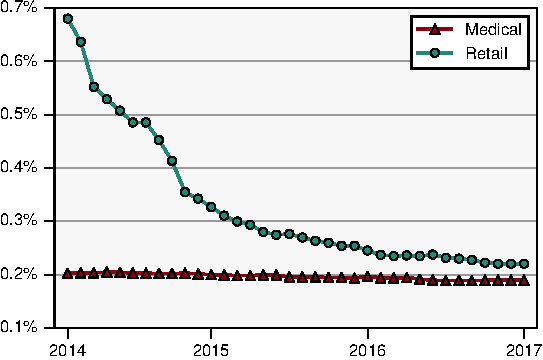
\includegraphics[scale=0.75]{images/market_share.pdf}\\
{\tiny Data Source: Colorado Department of Revenue.}
\end{center}


The concentration of firms in cannabis markets over time is of interest to participants in the cannabis industry, so, we will attempt to estimate a measure of market concentration and see if this measure changes over time.
\end{frame}

\section{Theory}

\begin{frame}{}
The \textbf{Herfindahl–Hirschman Index} (HHI) is a commonly accepted measure of market concentration. The HHI is calculated by squaring the market share of each firm competing in the market and then summing the resulting numbers.

\vspace{\baselineskip}
For example, for a market consisting of two firms with shares of 50 percent, the HHI is:
$$
50^2 + 50^2 = 5,000.
$$
\end{frame}


\begin{frame}{}
About the HHI metric:
\begin{itemize}
\item The HHI takes into account the relative size distribution of the firms in a market.
\item HHI approaches 0 when a market is occupied by a large number of firms of relatively equal size and reaches its maximum of 10,000 points when a market is controlled by a single firm.
\item The HHI increases both as the number of firms in the market decreases and as the disparity in size between those firms increases.
\end{itemize}
\end{frame}


\begin{frame}{}
Applications of the HHI in the legal system:
\begin{itemize}
\item The agencies generally consider markets in which the HHI is between 1,500 and 2,500 points to be moderately concentrated, and consider markets in which the HHI is in excess of 2,500 points to be highly concentrated.
\item Transactions that increase the HHI by more than 200 points in highly concentrated markets are presumed likely to enhance market power.
\end{itemize}
\end{frame}


%------------------------------------------------------------------%
% Takeaway
%------------------------------------------------------------------%

\begin{frame}{}
\begin{center}
\begin{minipage}{3.85in}
Thank you for coming.
\end{minipage}
\end{center}
\end{frame}

%------------------------------------------------------------------%
\end{document}
%------------------------------------------------------------------%